\documentclass[10pt]{article}
\usepackage{graphicx}
\usepackage{amssymb}
\usepackage[fleqn]{amsmath}
\usepackage{nccmath}
\usepackage{cases}
\usepackage{hyperref}
\usepackage{multicol}
\usepackage{tikz}
\usepackage{pgfplots}
\usepackage{enumitem}
\usepackage{pdfpages}
\pgfplotsset{compat=1.18}
\usepackage{float}

\title{\bf Math 151b: Problem Set 2}
\date{1/24/2024}
\author{\bf Owen Jones}
\begin{document}
\maketitle
\begin{enumerate}[label=\bf{Problem \arabic*}]
    \item Let $y'(t)=f(t,y(t))$.\\
    BE\@: $y_{n+1}=y_n+hf(t_{n+1},y_{n+1})$\\
    Note: let $f_t=f_t(\xi_1,\xi_2),f=f(t_n,y_n),f_y=f_y(\xi_1,\xi_2)$\\
    Taylor expand $f(t,y(t))$ about $(t_n,y_n)$ we obtain:\\
    $f(t_{n+1},y_{n+1})=f(t_n+h,y_n+hf(t_n,y_n))=f(t_n,y_n)+h(f_t+ff_y)$\\
    $y(t_{n+1})=y(t_n+h)=y(t_n)+hy'(t_n)+\frac{h^2y''(\xi_3)}{2}$\\
    The LTE for the Backward Euler method is:\\
    $\tau_{n+1}=y(t_{n+1})-y_{n+1}$ assuming $y(t_n)=y_n$.\\
    It follows $\tau_{n+1}=y(t_{n+1})-y_{n+1}\\
    =[y(t_n)+hy'(t_n)+\frac{h^2y''(\xi_3)}{2}]-\{y_n+h[f(t_n,y_n)+h(f_t+ff_y)]\}\\
    =[y(t_n)-y_n]+h[y'(t_n)-f(t_n,y_n)]+h^2[\frac{y''(\xi_3)}{2}-(f_t+ff_y)]\\
    =h^2[\frac{y''(\xi_3)}{2}-(f_t+ff_y)]=O(h^2)$\\
    Because $\tau_{n+1}$ is $O(h^2)$, the method is first order accurate.
    \item Maclaurin expansion for $e^x=1+x+\frac{x^2e^\xi}{2}$ for some $\xi$ between $0$ and $x$. 
    It follows $1+x\le e^x$ because $0\le \frac{x^2e^\xi}{2}$ which follows from $e^x\ge0$ for all $x$ and that the square of any number is nonnegative.
    Thus, for $x\ge-1$, we obtain $0\le 1+x\le e^x$.
    Because $0\le x\le y\Rightarrow 0\le x^n\le y^n$ for $n>0$ we have $0\le {(1+x)}^m\le e^{mx}$.
    \item \begin{enumerate}
        \item Proof by induction:
        Base case: $e_1\le(1+s)e_0+\theta=(1+s)\cdot 0+\theta=\theta$\\
        Induction hypothesis: $\displaystyle e_n\le \theta\sum_{k=0}^{n-1}{(1+s)}^k$ for some $n\ge 1$\\
        Induction step: $\displaystyle e_{n+1}\le (1+s)e_n+\theta\le \theta(1+s)\sum_{k=0}^{n-1}{(1+s)}^k+\theta\text{ (by the induction hypothesis)}\\
        =\theta\sum_{k=0}^{n}{(1+s)}^k$\\
        Hence, by induction,  $\displaystyle e_n\le \theta\sum_{k=0}^{n-1}{(1+s)}^k$ for all $n$.
        \item $\theta\sum_{k=0}^{n-1}{(1+s)}^k=\theta\frac{1-{(1+s)}^{n-1+1}}{1-(1+s)}=\frac{\theta}{s}({(1+s)}^{n}-1)$ by the sum of a geometric series.
        \item Using the result from problem $2$, we obtain $e_n\le\frac{\theta}{s}({(1+s)}^{n}-1)\le \frac{\theta}{s}(e^{ns}-1)$
    \end{enumerate}
    \item Applying the product rule and the chain rule,\\ 
    $\frac{\partial}{\partial t}(f_t)=\frac{\partial f_t}{\partial t}\frac{\partial t}{\partial t}+\frac{\partial f_t}{\partial y(t)}\frac{\partial y(t)}{\partial t}=f_{tt}+f_{ty}f,\\
    \frac{\partial}{\partial t}(ff_y)=ff_{yt}+(f_t+ff_y)f_y=f_t f_y+f{(f_y)}^2+ff_{ty}+f^2f_{yy}\\
    \Rightarrow \frac{\partial}{\partial t}y''(t)=\frac{\partial}{\partial t}(f_t+ff_y)=\frac{\partial}{\partial t}(f_t)+\frac{\partial}{\partial t}(ff_y)\\
    =f_{tt}+ff_{ty}+f_t f_y+f{(f_y)}^2+ff_{ty}+f^2f_{yy}\\
    =f_{tt}+2ff_{ty}+f^2f_{yy}+f_y(f_t+ff_y)$
    \item \begin{enumerate}
        \item Let $y(t)=\frac{1}{t}\Rightarrow y'(t)=-\frac{1}{t^2}$\\
        Thus, $y'(t)=-5y^2t+\frac{5}{t}-\frac{1}{t^2}=-5t\frac{1}{t^2}+\frac{5}{t}-\frac{1}{t^2}=-\frac{1}{t^2}$ which shows $y(t)=\frac{1}{t}$ is a solution to the IVP.
        \item 
        The second order Taylor Series of $y(t)$ centered at $t_n$ is:\\ 
        $y(t_n+h)=y(t_n)+h y'(t_n)+\frac{h^2y''(t_n)}{2}+\frac{h^3y'''(\xi)}{6}\\
        =y(t_n)+h f(t_n,y(t_n))+\frac{h^2}{2}(f_t(t_n.y(t_n))+f(t_n,y(t_n))f_y(t_n.y(t_n)))+O(h^3)$\\
        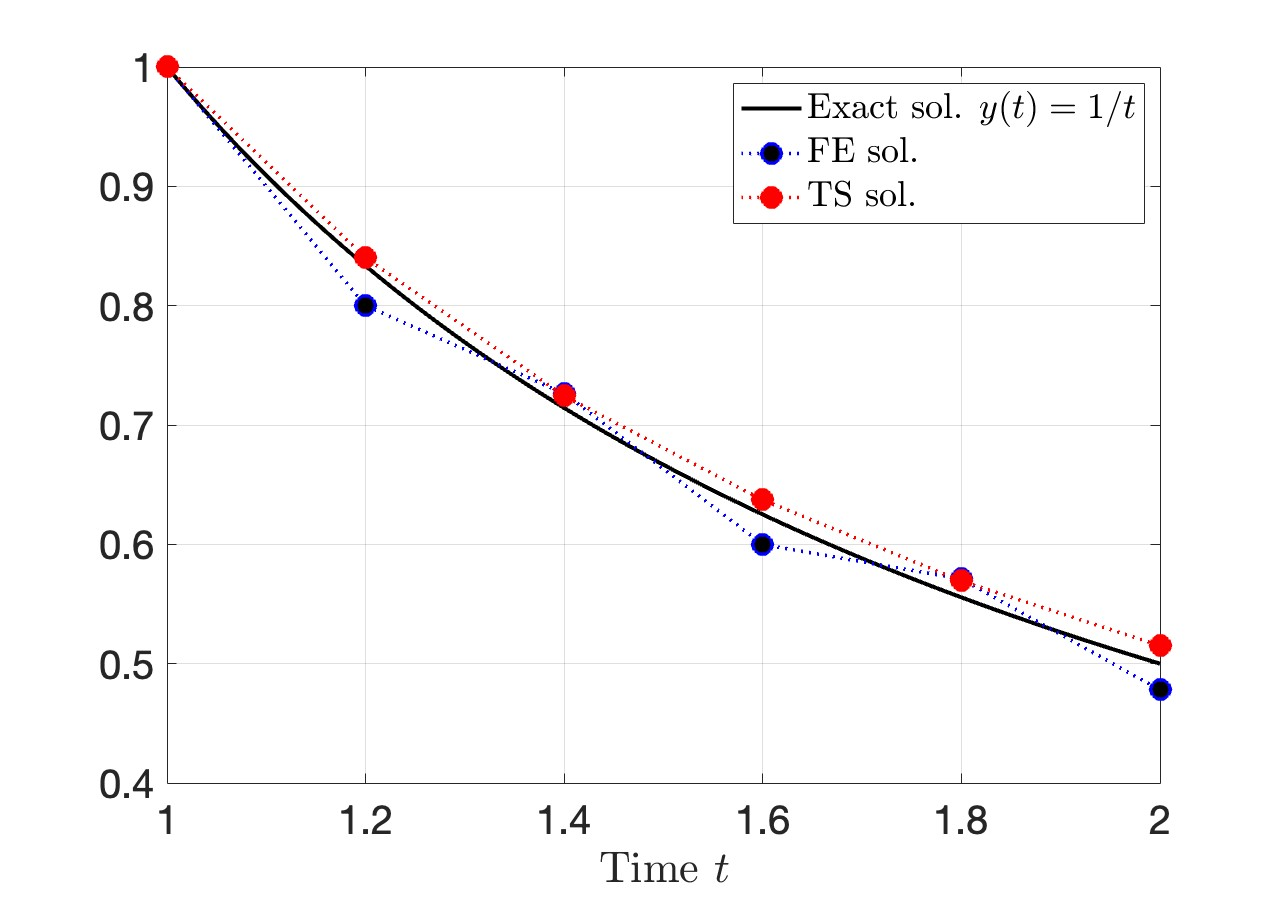
\includegraphics[scale=0.3]{homework_2_q5.jpg}
        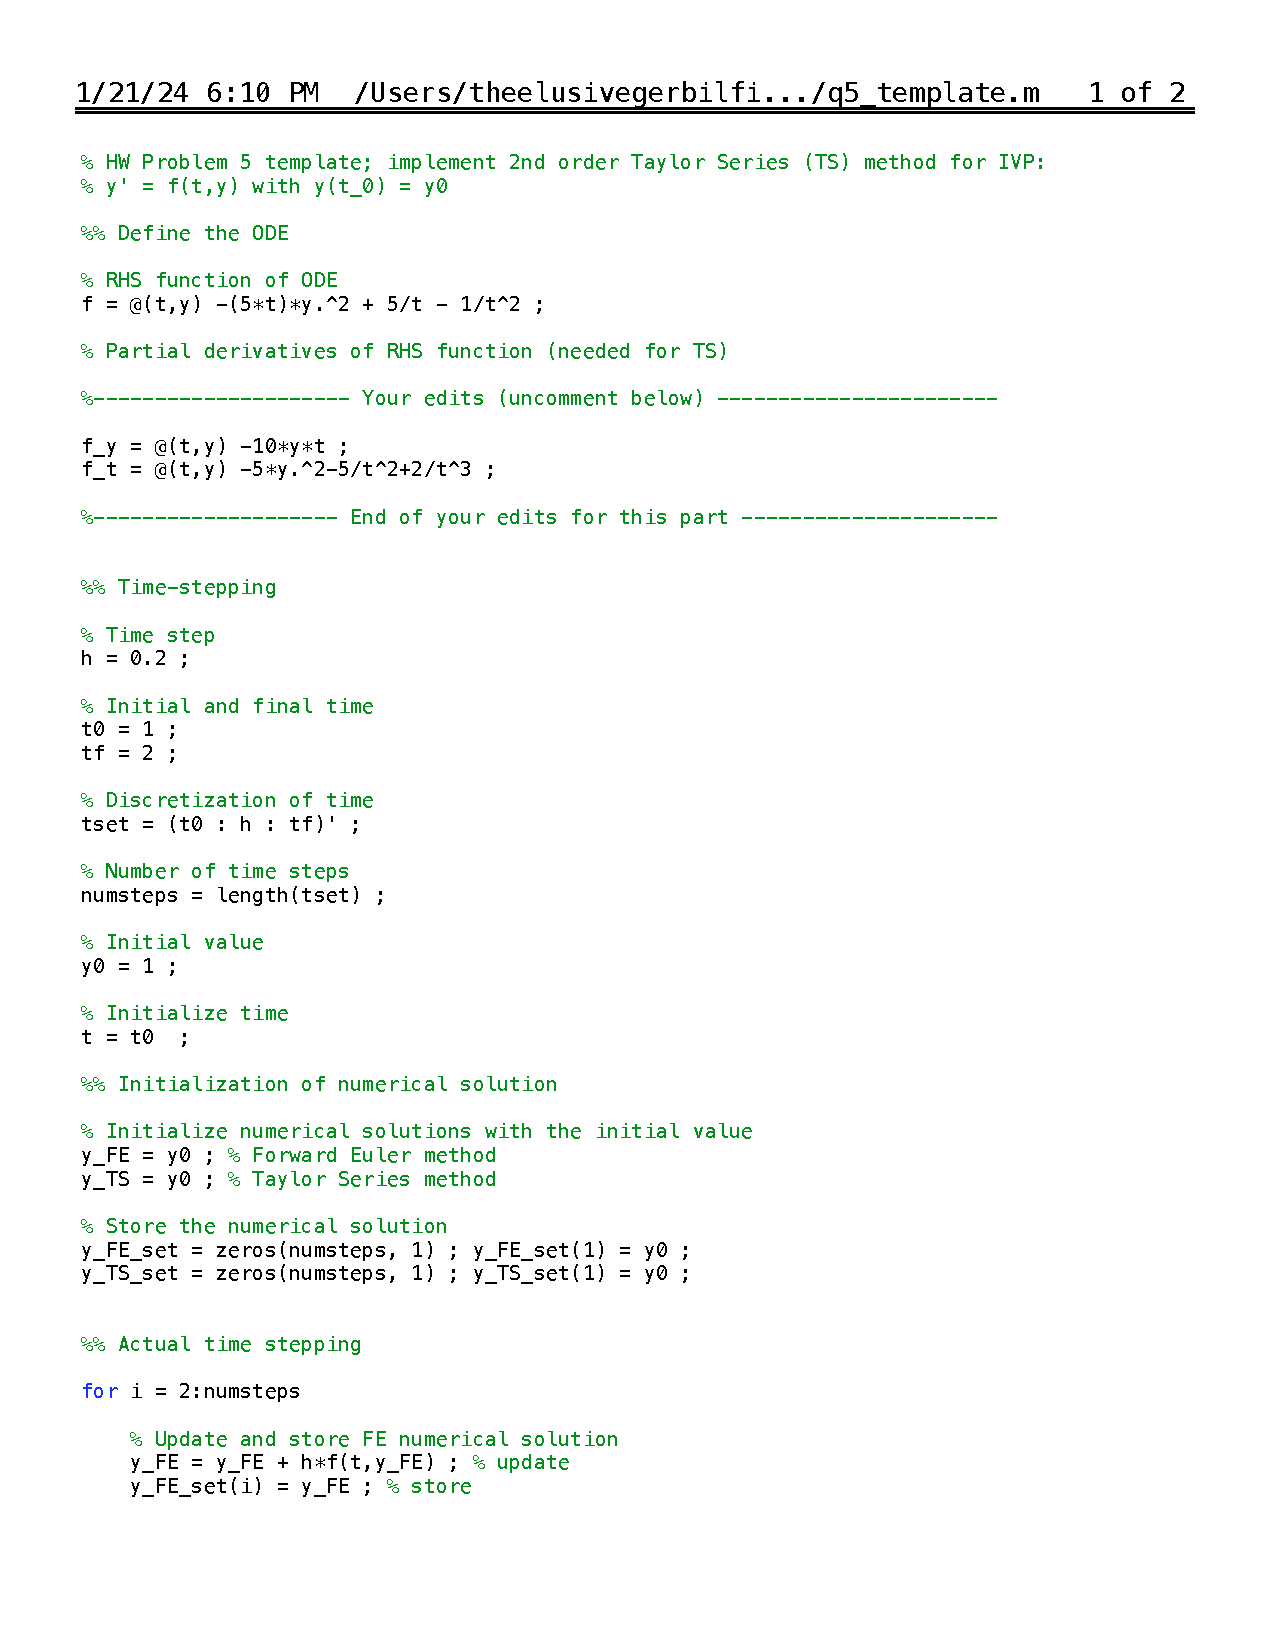
\includepdf[pages=-]{homework_2_q5_code.pdf}
    \end{enumerate}
\end{enumerate}
\end{document}